\documentclass[10pt]{article}
\usepackage[framemethod=TikZ]{mdframed}
\usepackage{amsthm}
\usepackage[landscape]{geometry}
\usepackage{multicol}
\usepackage{tikz}
\usepackage{pgfplots}
\usepackage{xcolor}
\usepackage{amsmath}
\usepackage[T1]{fontenc}
\usepackage{utopia}
\usepackage{changepage}
\usepackage{amssymb}
\usepackage{fancyhdr}
\usepackage[many]{tcolorbox}
\usepackage{moresize}
\usepackage{fullpage}
\usepackage{mathpazo}
\usepackage{tikz-3dplot}
\usepackage{cancel}
\tdplotsetmaincoords{70}{165}
\pgfplotsset{compat=1.18}

\usetikzlibrary{
    shadings, calc, patterns, angles, quotes, arrows.meta, 
    decorations.pathmorphing, decorations.pathreplacing, 
    fadings, 3d, perspective, backgrounds, intersections, 
    decorations.markings, bending
}

\tikzset{
    arrow/.style={-stealth,thick},
    node/.style={draw,thick,minimum size=6mm},
    label/.style={font=\small,inner sep=2pt},
    grid/.style={help lines,g},
    axis/.style={arrow,every node/.style={font=\small}},
    technical/.style={
        font=\small,
        tdplot_main_coords,
        anchor=center,
        inner sep=3pt
    },
    process/.style={
        scale=0.6,
        yscale=0.8,
        every node/.style={font=\small}
    },
    factor/.style={
        xscale=0.6,
        yscale=0.35,
        every node/.style={font=\small}
    }
}

\newcommand{\drawgrid}[4]{
    \foreach \x in {#1,...,#2} {
        \foreach \y in {#3,...,#4} {
            \draw[grid] (\x,\y) grid (\x+1,\y+1);
        }
    }
}

\newcommand{\drawaxes}[5]{
    \draw[#5] (0,0) -- (#1,0) node[right] {#3};
    \draw[#5] (0,0) -- (0,#2) node[above] {#4};
}

\newcommand{\drawpoint}[4]{
    \node[#4] at (#1,#2) {};
    \node[label] at (#1,#2) [right] {#3};
}

\newcommand{\drawstage}[5]{
    \draw[#1] (#2,#4) rectangle (#3,#4+1) node[midway] {#5};
}

\usepgfplotslibrary{
    groupplots, external, colormaps, patchplots, fillbetween
}

\setlength{\baselineskip}{1.2em}
\setlength{\parskip}{-0.75em}

\makeatletter
\tikzoption{canvas is xy plane at z}[]{%
    \def\tikz@plane@origin{\pgfpointxyz{0}{0}{#1}}%
    \def\tikz@plane@x{\pgfpointxyz{1}{0}{#1}}%
    \def\tikz@plane@y{\pgfpointxyz{0}{1}{#1}}%
    \tikz@canvas@is@plane}
\makeatother

% Reds (r)
\definecolor{r1}{RGB}{255, 191, 191}    % Light coral
\definecolor{r2}{RGB}{255, 191, 223}    % Light pink
\definecolor{r3}{RGB}{255, 207, 207}    % Light rose

% Blues (b)
\definecolor{b1}{RGB}{191, 223, 255}    % Light blue
\definecolor{b2}{RGB}{191, 239, 255}    % Light sky
\definecolor{b3}{RGB}{191, 255, 255}    % Light cyan

% Greens (g)
\definecolor{g1}{RGB}{191, 255, 191}    % Light green
\definecolor{g2}{RGB}{191, 255, 223}    % Light mint
\definecolor{g3}{RGB}{207, 255, 207}    % Light sage

% Oranges (o)
\definecolor{o1}{RGB}{255, 223, 191}    % Light peach
\definecolor{o2}{RGB}{255, 239, 191}    % Light cream
\definecolor{o3}{RGB}{255, 231, 191}    % Light buff

% Violets (v)
\definecolor{v1}{RGB}{223, 191, 255}    % Light purple
\definecolor{v2}{RGB}{239, 191, 255}    % Light lilac
\definecolor{v3}{RGB}{231, 191, 255}    % Light lavender

% Yellows (y)
\definecolor{y1}{RGB}{255, 255, 191}    % Light yellow
\definecolor{y2}{RGB}{255, 247, 191}    % Light cream yellow
\definecolor{y3}{RGB}{255, 239, 191}    % Light warm cream

\definecolor{w}{HTML}{eeeeee}
\definecolor{g}{HTML}{444444}
\definecolor{b}{HTML}{222222}
\definecolor{lightgrey}{HTML}{cccccc}

\geometry{
    letterpaper,
    left=0.25in,
    right=0.25in,
    top=0.15in,
    bottom=0.25in
}

\newcommand{\hr}{\centerline{\rule{3.5in}{1pt}}}

\newcommand{\nc}[2][b]{%
\tikz \draw [draw=#1,thick]
    ($(current page.center)-(0.495\linewidth,0)$) -- 
    ($(current page.center)+(0.495\linewidth,0)$)
    node [midway, fill=b] {\ssmall\textbf{\uppercase{#2}}};
}

\newtcolorbox{conceptbox}[2][]{
	breakable,
	vfill before first=false,
	segmentation at break=false,
	size=fbox,
	colback=b,
	title=\scriptsize\textbf{\MakeUppercase{#2}},
	left=2pt,
	right=2pt,
	top=3pt,
	bottom=1pt,
	boxrule=1pt,
	coltitle=b,
	colupper=w,
	pad at break=5pt,
	toprule at break=4pt,
	bottomrule at break=0.75pt,
	colframe=#1,
	enlargepage=12in, 
	before upper*={\setlength{\baselineskip}{0.75em}\setlength{\parskip}{0em}}
}

\title{TEMPLATE}
\parindent0pt

\begin{document}
\ssmall
\pagecolor{b}
\fontfamily{put}
\begin{minipage}{\textwidth} %title
	\tikz{
		\draw[thick, color=w] (1,0) -- (\textwidth-0.25in,0);
		\node[anchor=west, fill = b, inner sep = 3pt, text=w] at (0,0) {\textbf{TEMPLATE}};
		\node[anchor=east, fill = b, inner sep = 3pt, text=w] at (\textwidth,0) {\textbf{NAME}};
	}
\end{minipage}

\begin{multicols*}{4}
	\begin{conceptbox}[v3]{Header 1}
		\nc[v3]{Header 2}
	\end{conceptbox}

	\begin{conceptbox}[r3]{Header 1}
		\nc[r3]{Header 2}
	\end{conceptbox}

	\begin{conceptbox}[o3]{Header 1}
		\nc[o3]{Header 2}
	\end{conceptbox}

	\begin{conceptbox}[b3]{Header 1}
		\nc[b3]{Header 2}
	\end{conceptbox}
	\columnbreak
	\begin{conceptbox}[w]{Tikz Diagrams}
		\tiny
		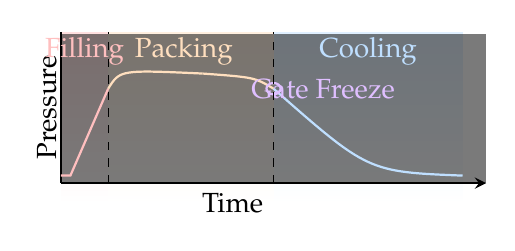
\begin{tikzpicture}[scale=0.6, yscale=0.8]
			\fill[color=r1, draw opacity=0.5, fill opacity=0.5, path fading=south] (0,-0.5) rectangle (1,4);
			\fill[o1, draw opacity=0.5, fill opacity=0.5, path fading=south] (1,-0.5) rectangle (4.5,4);
			\fill[b1, draw opacity=0.5, fill opacity=0.5, path fading=south] (4.5,-0.5) rectangle (8.5,4);
			\fill[color=b, fill opacity=0.6] (0,0) rectangle (9,3.95);
			\draw[-stealth, thick] (0,0) -- (9,0) node[below left, midway]{Time};
			\draw[-, thick] (0,0) -- (0,4) node[rotate=90, anchor=center] at (-0.3,2) {Pressure};
			\draw[r1,thick] (0,0.2) -- (0.2,0.2) -- (1,2.5);
			\draw[o1,thick] (1,2.5) .. controls (1.25,3) .. (3,2.9);
			\draw[o1,thick] (3,2.9) .. controls (4.1,2.8) .. (4.5,2.5);
			\draw[b1,thick] (4.5,2.5) .. controls (6.5,0.3) .. (8.5,0.2);
			\node[r1] at (0.5,3.5) {Filling};
			\node[o1] at (2.6,3.5) {Packing};
			\node[b1] at (6.5,3.5) {Cooling};
			\draw[v1,thick] (4.5,2.5) circle (0.15);
			\node[v1] at (5.55,2.5) {Gate Freeze};
			\draw[dashed] (1,0) -- (1,4);
			\draw[dashed] (4.5,0) -- (4.5,4);
		\end{tikzpicture}\\[1em]
		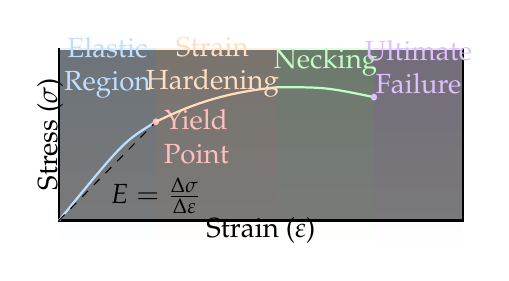
\begin{tikzpicture}[scale=0.57, yscale=1.1]
			\fill[color=b1, draw opacity=0.5, fill opacity=0.5, path fading=south] (0,-0.5) rectangle (2.16,3.5);
			\fill[o1, draw opacity=0.5, fill opacity=0.5, path fading=south] (2.16,-0.5) rectangle (4.86,3.5);
			\fill[g1, draw opacity=0.5, fill opacity=0.5, path fading=south] (4.86,-0.5) rectangle (7.02,3.5);
			\fill[v1, draw opacity=0.5, fill opacity=0.5, path fading=south] (7.02,-0.5) rectangle (9,3.5);
			\fill[color=b, fill opacity=0.6] (0,0) rectangle (9,3.45);
			\draw[-,thick] (0,3.5) -- (0,0) -- (9,0) -- (9,3.5);
			\node at (4.5,-0.2) {Strain ($\varepsilon$)};
			\node[rotate=90] at (-0.2,1.75) {Stress ($\sigma$)};
			\draw[b1,thick] (0,0) .. controls (1.44,1.6) .. (2.16,2);
			\node[b1, align=center] at (1.08,3.1) {Elastic\\Region};
			\draw[dashed] (0,0) -- (2.16,2);
			\node at (2.16,0.5) {$E = \frac{\Delta\sigma}{\Delta\varepsilon}$};
			\fill[r1] (2.16,2) circle (2pt);
			\node[r1, align=center] at (3.06,1.7) {Yield \\Point};
			\draw[o1,thick] (2.16,2) .. controls (3.06,2.4) and (3.78,2.6) .. (4.86,2.7);
			\node[o1, align=center] at (3.42,3.1) {Strain\\Hardening};
			\draw[g1,thick] (4.86,2.7) .. controls (5.94,2.7) .. (7.02,2.5);
			\node[g1] at (5.94,3.2) {Necking};
			\fill[v1] (7.02,2.5) circle (2pt);
			\node[v1, align=center] at (8.01,3.1) {Ultimate\\Failure};
		\end{tikzpicture}\\[0.5em]
		\begin{center}
		\begin{tikzpicture}[
			font = \tiny \boldmath,
			tdplot_main_coords,
			anchor=center,
			inner sep = 3pt,
			axis/.style={->,blue,line width=0.8pt},
			cube/.style={},
			scale=0.9,
			face/.style={cube,line width=0.6pt,draw=w},
			filled face/.style={face,fill=b!90,opacity=0.8},
			arrow style/.style={-stealth,line width=0.5pt},
		]

		\def\gridrange{1.7,2.07,2.43,2.8}
		\def\zrange{0.2,0.57,0.93,1.3}

		\begin{scope}[shift={(-0.2,0,-1.5)}, scale=0.8]
			\draw[-stealth] (0,0,0) -- (0.5,0,0) node[scale=0.9, anchor=east] {x};
			\draw[-stealth] (0,0,0) -- (0,0.7,0) node[scale=0.9, anchor=north east] {y};
			\draw[-stealth] (0,0,0) -- (0,0,0.4) node[scale=0.9, anchor=south] {z};
		\end{scope}

		\draw[cube, fill=b2, opacity=.5] (1.5,1.5,-0.3) -- (3,1.5,-0.3) -- (3,3,-0.3) -- (1.5,3,-0.3) -- cycle;
		\draw[cube,thick,draw=b2] (1.5,1.5,-0.3) -- (3,1.5,-0.3) -- (3,3,-0.3) -- (1.5,3,-0.3) -- cycle;

		\begin{scope}[opacity=0.8]
			\draw[cube, fill=b] (1.1,1.5,0) -- (1.1,3,0) -- (1.1,3,1.5) -- (1.1,1.5,1.5) -- cycle;
			\draw[cube, fill=r2!90, opacity=.4] (1.1,1.5,0) -- (1.1,3,0) -- (1.1,3,1.5) -- (1.1,1.5,1.5) -- cycle;
			\draw[cube,thick,draw=r2] (1.1,1.5,0) -- (1.1,3,0) -- (1.1,3,1.5) -- (1.1,1.5,1.5) -- cycle;
		\end{scope}

		\draw[cube, fill=b, draw=b] (1.5,1.5,0) -- (1.5,3,0) -- (1.5,3,1.5) -- (1.5,1.5,1.5) -- cycle;

		\foreach \face in {
				{(1.5,1.5,0) -- (3,1.5,0) -- (3,1.5,1.5) -- (1.5,1.5,1.5)},
				{(1.5,1.5,0) -- (1.5,3,0) -- (1.5,3,1.5) -- (1.5,1.5,1.5)},
				{(1.5,1.5,0) -- (1.5,3,0) -- (3,3,0) -- (3,1.5,0)}
			} {
				\draw[cube,thick,draw=w, fill=b!90] \face;
			}

		\foreach \y in \gridrange {
			\foreach \z in \zrange {
				\draw[arrow style, r2, opacity=((\y-1.4)/1.5 + (\z+0.5)/1.5)/2]
				(0.6,\y,\z) -- (3.6,\y,\z);
			}
		}

		\foreach \x in \gridrange {
			\foreach \y in \gridrange {
				\draw[arrow style, b2, opacity={((\y-1.7)/1.1 + (\x-1.7)/1.1)/2}]
				(\x,\y,-0.7) -- (\x,\y,2);
			}
		}

		\foreach \face in {
				{(1.5,3,0) -- (3,3,0) -- (3,3,1.5) -- (1.5,3,1.5)},
				{(1.5,1.5,1.5) -- (1.5,3,1.5) -- (3,3,1.5) -- (3,1.5,1.5)},
				{(3,1.5,0) -- (3,3,0) -- (3,3,1.5) -- (3,1.5,1.5)}
			} {
				\draw[filled face] \face;
				\draw[face] \face;
			}

		\foreach \x in \gridrange {
			\foreach \y in \gridrange {
				\draw[arrow style, draw=b2,
					opacity={((\y-1.5)/1.1 + (\x-1.6)/1.1)/2.1}]
				(\x,\y,1.5) -- (\x,\y,2);
			}
		}
		\foreach \y in \gridrange {
			\foreach \z in \zrange {
				\draw[arrow style, draw=r2,
					opacity={((\y-1.5)/1.1 + (\z-0.1)/1.1)/2.1}]
				(3,\y,\z) -- (3.6,\y,\z);
			}
		}

		\begin{scope}[canvas is xz plane at y=2.25]
			\node[scale=1.1, text=r2, inner sep=2pt, xscale=-1, transform shape] at (0.1,0.6) {$u_x\Delta y\Delta z$};
		\end{scope}

		\begin{scope}[canvas is xz plane at y=2.25]
			\node[scale=1.1, text=r2, inner sep=2pt, xscale=-1, transform shape] at (4.5,0.55) {$(u_x+\Delta u_x)\Delta y\Delta z$};
		\end{scope}

		\begin{scope}[canvas is xz plane at y=3]
			\node[scale=1.1, text=b2,fill=b, inner sep=2pt, xscale=-1, transform shape] at (2.27,-0.5) {$u_y\Delta x\Delta z$};
		\end{scope}

		\begin{scope}[canvas is xz plane at y=2.25]
			\node[scale=1.1, text=b2, inner sep=2pt,  xscale=-1, transform shape] at (2.25,2.4) {$(u_y+\Delta u_y)\Delta x\Delta z$};
		\end{scope}
		\end{tikzpicture}
	\end{center}
	\end{conceptbox}
\end{multicols*}
\end{document}
